\documentclass[a4paper, 12pt]{article}

\usepackage[T1]{fontenc}
\usepackage[utf8]{inputenc}

\usepackage{roboto}
\usepackage{parskip}
\usepackage[english]{babel}
\usepackage{a4wide}
\usepackage{graphicx}
\usepackage{svg}

\title{intelliPhoto - Manual}
\author{Paul Norberger \& the intelliPhoto team}

\begin{document}
\begin{titlepage}
\maketitle
\thispagestyle{empty}
\begin{center}
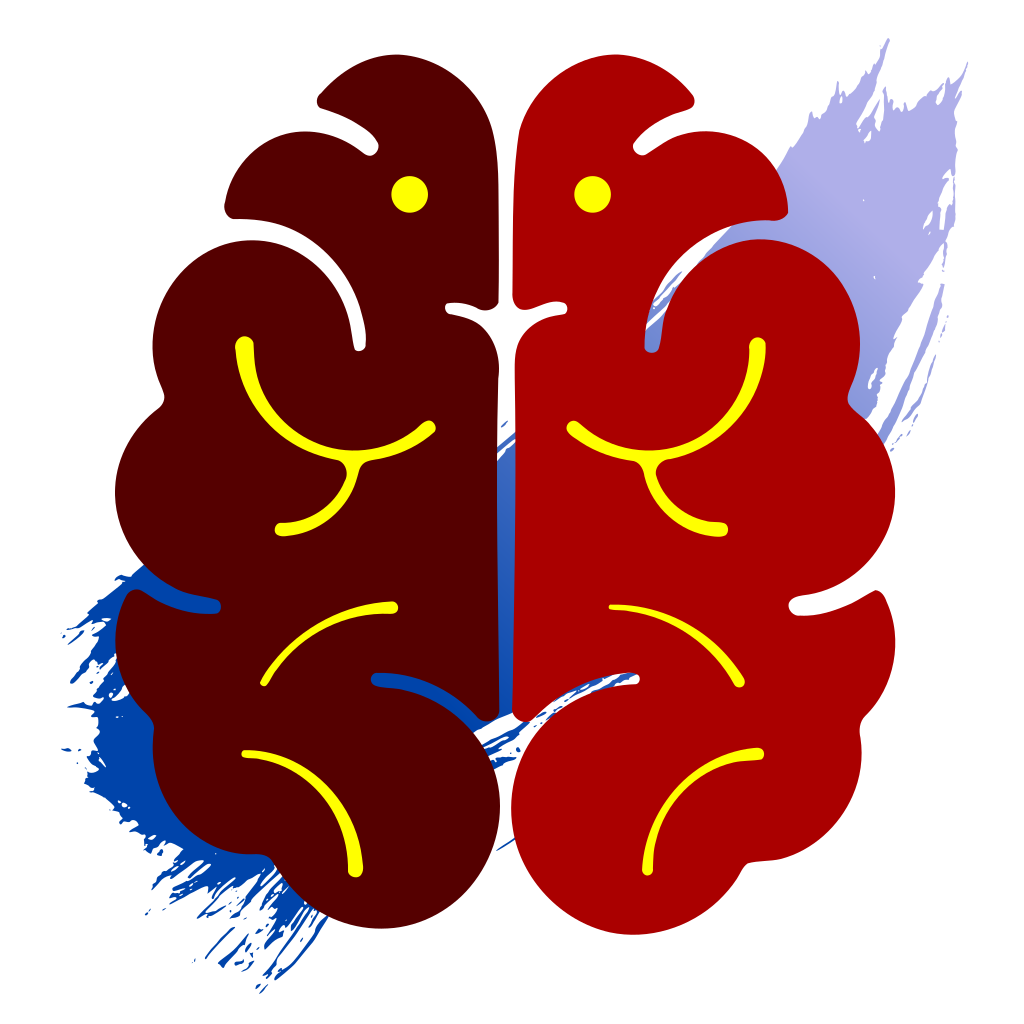
\includegraphics[width=0.45\linewidth,keepaspectratio]{assets/icon}
\end{center}
\tableofcontents
\end{titlepage}
\section{Introduction}
intelliPhoto is a software for creating and editing graphics of various kinds. While it allows for work with a full color space, it will also allow export in a more restriced format, which uses 1 byte per pixel. Currently its in its early stages of development and has a very limited array of tools as well as a functional, but barebones interface. This will change in future versions.
Currently the following features are implemented, which will be described in further detail on the following pages:
\begin{itemize}
\item A barebones user interface
\item Loading and Saving images from and to standardized formats (such as .png, .bmp or .jpg)
\item Drawing with a pen tool with adjustable width and color
\item A layer structure, that allows for moving layers and changing the order of them as well as multiple layer types:
\item Shaped Layers, described with a polygon that allow for transparency
\item Raster Layers, that fill the whole canvas and do not use transparecy.
\end{itemize}

\section{User Guide}
After startup the following window opens:
\begin{center}
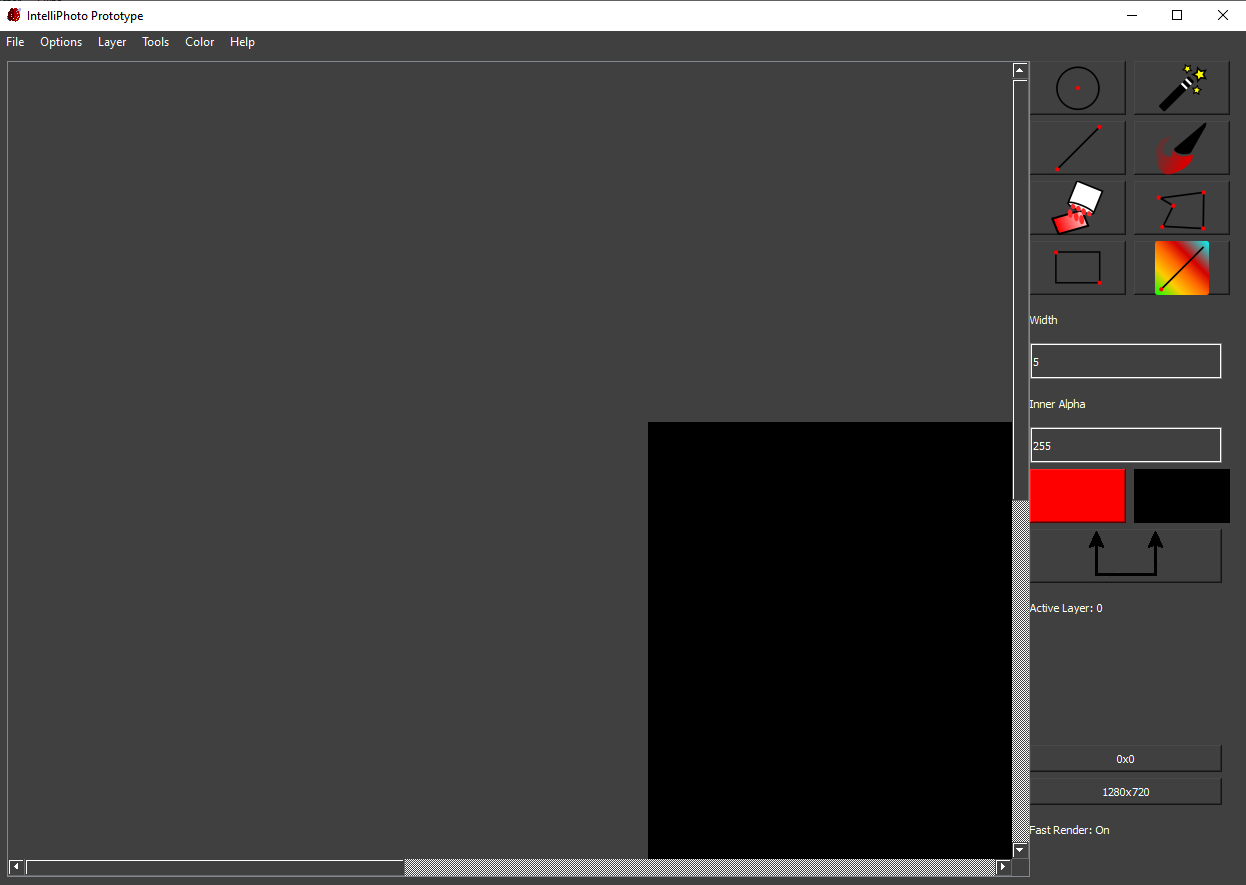
\includegraphics[width=0.5\linewidth,keepaspectratio]{assets/startup}
\end{center}

\subsection{Loading images}

To load a preexisting image, click on "File" in the top menu bar and then on "Open..." in the appearing context menu.
\begin{center}
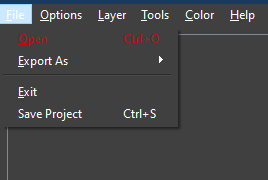
\includegraphics[width=0.3\linewidth,keepaspectratio]{assets/file-open}
\end{center}

A file explorer window opens. Navigate to the image you want to open and click on "Open" or the equivalent in your system language. The image will now be imported and displayed.

\subsection{Saving images}
To save the current canvas as an image, click on "File" in the top menu bar then hover over "Save As" and click on your preferred file format in the appearing context menu.
\begin{center}
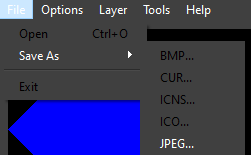
\includegraphics[width=0.3\linewidth,keepaspectratio]{assets/file-save}
\end{center}

A file explorer window opens. Navigate to your preferred save location, input a file name and click on "Save" or the equivalent in your system language. The image will be saved at that location in the selected file format.

\subsection{Setting the active layer}
The active layer is the layer you are currently editing. To change it, you currently have to specify the index of the layer under "Active:" on the righ side of the canvas and then click on "select Active". Since there is currently no way to create or delete layers the program opens with 2 layers by default: One ShapedImage (the triange) and one raster image (the square), you can switch between these at any times by doing the described steps.
Only 0 and 1 are valid 'Active:' values because of this.

\subsection{Setting width and color of the pen}
To edit width and color of the drawing tool, click on "Options" in the top menu bar then select either "Pen Color..." or "Pen Width..." depending on which parameter you want to edit.
\begin{center}
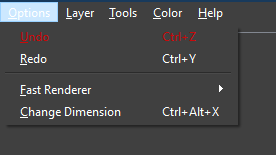
\includegraphics[width=0.3\linewidth,keepaspectratio]{assets/file-options}
\end{center}
In the appearing popup you can select a new value for the parameter.

\subsection{Drawing with the pen tool}
To edit the active layer with the pen tool simply click and hold the left mouse button while hovering the layer on the canvas. When you click within the boundaries of the active layer, the pixels in the radius you selected will change their color to the color which you selected under the section above.

\subsection{Fill the active layer in one color}
To fill the whole layer with one specific color, you first specify the color on the right side of the picture.

Afterwards you click on the "set Color" button above the color specification fields.
\begin{center}
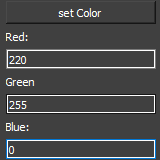
\includegraphics[width=0.3\linewidth,keepaspectratio]{assets/fill-layer}
\end{center}

\subsection{Moving layers}
The layers are flexible and can be moved to a different position on the canvas, their order can be changed at will. For this you can use the buttons on the bottom of the right side panel. Keep in mind that the changes always only effect the active layer you have chosen in the section "Setting the active layer".

\begin{center}
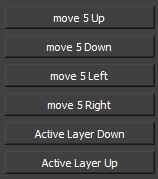
\includegraphics[width=0.3\linewidth,keepaspectratio]{assets/moving-layers}
\end{center}

\subsection{Transparency and layers}
Layers can also be made more or less transparent by entering a value under "Alpha:" on the right side of the canvas. Values between 0 and 255 are valid. There is currently no error handling and this can lead to memory leaks, so be careful. This also only effects the active layer.

\begin{center}
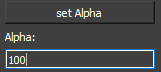
\includegraphics[width=0.3\linewidth,keepaspectratio]{assets/layer-alpha}
\end{center}

\section{Next steps}
The following features are currently high priority and will be implimented in the near future:
\begin{itemize}
\item Implementing a reusable, modular tool structure that makes it easy to implement future tools and make them compatible with other features such as the UI
\end{itemize}

\end{document}